\documentclass[11pt,a4paper]{article}
\usepackage[T1]{fontenc}
\usepackage[utf8]{inputenc}
\usepackage{libertinus}
\usepackage{amsmath,amssymb,amsthm,mathtools}
\usepackage[a4paper,margin=27mm,headheight=15pt]{geometry}
\usepackage{microtype,booktabs,array,longtable}
\usepackage{enumitem,tikz,fancyhdr,xcolor}
\usepackage[most]{tcolorbox}
\usepackage{hyperref}
\usepackage[nameinlink,noabbrev]{cleveref}
\hypersetup{colorlinks=true,linkcolor=blue!45!black,citecolor=blue!45!black,
 urlcolor=blue!45!black,pdftitle={The Brownian Matrix Governing Fabius Smoothness},
 pdfauthor={Research report prepared for Vladimir Reshetnikov},
 pdfsubject={Sharp anisotropic Fourier envelopes and mixed derivative growth},
 pdfkeywords={Fabius function, common digits, Fourier decay, mixed derivatives, convex duality, resonance}}
\pagestyle{fancy}\fancyhf{}
\fancyhead[L]{\small Sharp smoothness of common-digit Fabius laws}
\fancyhead[R]{\small Research draft}
\fancyfoot[C]{\thepage}
\setlength{\parskip}{4pt}\setlength{\parindent}{1.2em}
\setlength{\emergencystretch}{2em}
\numberwithin{equation}{section}
\newtheorem{theorem}{Theorem}[section]
\newtheorem{lemma}[theorem]{Lemma}
\newtheorem{proposition}[theorem]{Proposition}
\newtheorem{corollary}[theorem]{Corollary}
\theoremstyle{definition}
\newtheorem{definition}[theorem]{Definition}
\newtheorem{example}[theorem]{Example}
\newtheorem{question}{Research question}
\theoremstyle{remark}\newtheorem{remark}[theorem]{Remark}
\newcommand{\R}{\mathbb R}\newcommand{\N}{\mathbb N}
\newcommand{\E}{\mathbb E}\newcommand{\Prob}{\mathbb P}
\newcommand{\dd}{\,\mathrm d}
\newcommand{\ii}{\mathrm i}
\newcommand{\one}{\mathbf 1}
\newcommand{\sinc}{\operatorname{sinc}}
\newcommand{\supp}{\operatorname{supp}}
\newcommand{\Vol}{\operatorname{Vol}}
\newcommand{\He}{\mathcal H}
\newcommand{\Qf}{\mathcal Q}
\newcommand{\lp}{\log_+}
\newcommand{\norm}[1]{\left\lVert #1\right\rVert}
\newcommand{\abs}[1]{\left|#1\right|}
\newcommand{\repo}{\textit{Common-Digit Fabius Zonoids}}
\newtcolorbox{resultbox}{enhanced,breakable,colback=black!2,colframe=black!40,
 boxrule=.4pt,arc=1mm,left=2mm,right=2mm,top=1mm,bottom=1mm}
\newcommand{\snapshot}{23dd71d2d3d5e85d2b97a8cc45f55e735d69a4ae}

\begin{document}
\begin{titlepage}
\vspace*{9mm}
\noindent{\large\scshape ProveIt research continuation}\par
\vspace{10mm}
\noindent{\Huge\bfseries The Brownian Matrix\\[3mm]Governing Fabius\\[3mm]Smoothness}\par
\vspace{7mm}
\noindent{\Large Sharp anisotropic Fourier envelopes,\\mixed derivative growth, and a signed resonance}\par
\vspace{10mm}
\noindent Research report prepared for Vladimir Reshetnikov\\
29 September 2026
\vspace{9mm}
\begin{abstract}
The common-digit geometric-uniform construction couples several Fabius-type
laws using one sequence of independent uniform digits. Its smooth joint density
is known in the ProveIt corpus, but sharp joint Fourier decay is left
conjectural. We prove a uniform logarithmic-box envelope for the joint infinite
sinc product, including matching lower bounds on a fixed positive proportion
of every box. The controlling function is the area under the upper envelope
of finitely many lines. Its positive-orthant convex conjugate is exactly the
quadratic form associated with the matrix
$M_{ij}=\min(\lambda_i,\lambda_j)$, where $\lambda_j=-\log|q_j|$.
Consequently, for every mixed derivative and every $1\le p\le\infty$,
\[
 \log\norm{\partial^\alpha f}_{L^p}
 =\frac12\alpha^{\mathsf T}M\alpha+O(|\alpha|+1),
\]
with an error uniform over all multi-indices and all such $p$.
This identifies the complete quadratic-order anisotropic smoothness law,
not just an isotropic upper estimate. We also prove sharp ray-window decay,
a reciprocal convolution-power law, directional derivative stratification,
and quantitative boundary flatness. Distinct parameter moduli are essential:
at the signed pair $(r,-r)$ the leading derivative-growth coefficient doubles.
The resulting discontinuity yields two noncommuting parameter/order limits.
All principal arguments are given in full. Exact finite algebra checks and
high-precision diagnostics accompany the article; the analytic proofs have
not been checked by a proof assistant.
\end{abstract}
\vfill
\noindent\small\textbf{Status.} Unrefereed research draft. The precise derivative law and
its multivariate envelope proof are contributions developed here relative to
the inspected source. No claim of exhaustive historical priority is made.
\end{titlepage}

\begingroup
\small
\setlength{\parskip}{0pt}
\tableofcontents
\endgroup
\clearpage

\section{The research gap and the principal results}
\label{sec:intro}

\subsection{What is already established, and what is new here}

For independent $U_k\sim\operatorname{Uniform}[0,1]$, the normalized variables
\begin{equation}
 X_q=(1-q)\sum_{k=0}^{\infty}q^kU_k,\qquad 0<q<1,
 \label{eq:normalized}
\end{equation}
provide the common-digit geometric-uniform family: the same $U_k$ is used at
each parameter. The one-dimensional $q=1/2$ law belongs to the classical
Fabius--Rvachev theory \cite{Fabius,Arias}. The repository report \repo\ already
proves its multivariate support formula, a joint infinite sinc product,
$C_c^\infty$ regularity, boundary flatness, and exact support volumes
\cite{Repo}. Those facts are not new claims of the present article.

The explicit unresolved item is the report's
\texttt{conj:ray-decay}, in the subsection ``Sharp ray-wise decay of the joint
sinc product.'' It predicts a quadratic logarithmic leading term determined
by the largest surviving parameter, while also proposing a more delicate
periodic/quasiperiodic description of the remainder. Its reference to
neighborhoods of the zero hyperplanes does not prescribe a precise exceptional
set. Our answer separates these issues. We prove the sharp leading envelope
with a precise window and measure formulation, then strengthen it to
frequency directions that move with scale. We do \emph{not} prove the proposed
periodic/quasiperiodic remainder description.

The main additional result is the exact mixed-derivative growth law. It
contains cross terms that are absent for independent marginals. These terms
are the analytic signature of sharing the same digits.

The source was inspected at commit \texttt{23dd71d2d3d5e85d2b97a8cc45f55e735d69a4ae}.
The relevant source labels are \texttt{thm:joint-char},
\texttt{thm:density-regularity}, and \texttt{conj:ray-decay}.
The package's \texttt{PROVENANCE.md} records the exact path and the inspection
boundary. A targeted search did not locate the mixed-derivative formula below
in the inspected report or the retrieved related material. That is a
bounded source comparison, not a claim to have searched all mathematical
literature.

\subsection{A normalization that exposes the Fourier geometry}

Let $V_k=2U_k-1$, so $V_k$ is uniform on $[-1,1]$. We use the centered variables
\begin{equation}
 Y_j=\sum_{k=0}^{\infty}q_j^kV_k,\qquad 1\le j\le d.
 \label{eq:Y}
\end{equation}
Unless explicitly stated otherwise, assume
\begin{equation}
 0<|q_j|<1,\qquad |q_i|\ne|q_j|\quad(i\ne j),\qquad
 \lambda_j=-\log|q_j|.
 \label{eq:assumptions}
\end{equation}
Thus signed parameters are allowed, but repeated moduli are not. Let $f$ be
the density of $Y=(Y_1,\ldots,Y_d)$. We prove its existence and smoothness below.
For the positive normalized family,
\begin{equation}
 X_{q_j}=\frac12+\frac{1-q_j}{2}Y_j.
 \label{eq:scale}
\end{equation}
Fixed nonzero diagonal changes of coordinates alter logarithms of derivative
norms by only $O(|\alpha|+1)$. Hence the leading results are identical for
\eqref{eq:normalized} and \eqref{eq:Y}.

Write
\begin{equation}
 M_{ij}=\min(\lambda_i,\lambda_j),\qquad
 \Qf(\alpha)=\frac12\alpha^{\mathsf T}M\alpha,
 \qquad |\alpha|=\sum_j\alpha_j.
 \label{eq:MQ}
\end{equation}
All logarithms are natural. Multi-indices belong to $\N^d$, with zero included
in $\N$. Constants may depend on the fixed parameter vector and on $d$; they
are not asserted to remain bounded as moduli collide.

\begin{theorem}[Sharp mixed-derivative law]
\label{thm:main}
Under \eqref{eq:assumptions}, $f\in C_c^\infty(\R^d)$. There exist $A,B\ge1$,
independent of $\alpha$ and $p$, such that for every $\alpha\in\N^d$ and
$1\le p\le\infty$,
\begin{equation}
 A^{-1}B^{-|\alpha|}\exp\Qf(\alpha)
 \ \le\ \norm{\partial^\alpha f}_{L^p}
 \ \le\ AB^{|\alpha|}\exp\Qf(\alpha).
 \label{eq:main-bounds}
\end{equation}
In particular,
\begin{equation}
 \boxed{\log\norm{\partial^\alpha f}_{L^p}
       =\frac12\sum_{i,j=1}^d
        \min(\lambda_i,\lambda_j)\alpha_i\alpha_j+O(|\alpha|+1).}
 \label{eq:main-log}
\end{equation}
If $\alpha^{(n)}/n\to a\in[0,\infty)^d$, then
\begin{equation}
 \frac1{n^2}\log\norm{\partial^{\alpha^{(n)}}f}_{L^p}
 \longrightarrow\frac12a^{\mathsf T}Ma.
 \label{eq:direction-alpha}
\end{equation}
The limit remains valid if $p$ varies with $n$ in $[1,\infty]$.
\end{theorem}

This is a two-sided result. In particular, the upper bound cannot be improved
by replacing the quadratic form with a strictly smaller value on any
nonnegative derivative direction.

\subsection{The Fourier statement behind the derivative law}

For $s\in[0,\infty)^d$ define
\begin{equation}
 \He(s)=\int_0^\infty \max\{0,s_1-\lambda_1u,\ldots,s_d-\lambda_du\}\dd u,
 \qquad S=\max_js_j.
 \label{eq:H}
\end{equation}
Let $\lp x=\max(0,\log x)$ for $x>0$, and set $\lp0=0$. The characteristic
function of \eqref{eq:Y} is
\begin{equation}
 \Phi(t)=\E e^{\ii t\cdot Y}
       =\prod_{k=0}^{\infty}\sinc\!\left(\sum_{j=1}^dt_jq_j^k\right),
 \qquad \sinc z=\begin{cases}\sin z/z,&z\ne0,\\1,&z=0.\end{cases}
 \label{eq:Phi}
\end{equation}
For a logarithmic scale vector $s$, put
\begin{equation}
 B_s=\prod_{j=1}^d[e^{s_j},2e^{s_j}].
 \label{eq:box}
\end{equation}
Averages on this box are with respect to its normalized Lebesgue measure.

\begin{theorem}[Uniform logarithmic-box envelope]
\label{thm:envelope}
There are constants $C_+,C_->0$ such that
\begin{align}
 \log|\Phi(t)|&\le-\He(\lp|t_1|,\ldots,\lp|t_d|)
                  +C_+(1+\max_j\lp|t_j|),\label{eq:upper-envelope}\\
 \frac1{\Vol B_s}\int_{B_s}\log|\Phi(t)|\dd t
       &\ge-\He(s)-C_-(1+S).\label{eq:mean-envelope}
\end{align}
The value $-\infty$ at a zero is permitted in the first inequality. The
integral in the second inequality is finite. Consequently,
\begin{equation}
 \log\sup_{t\in B_s}|\Phi(t)|=-\He(s)+O(1+S),
 \label{eq:boxsup}
\end{equation}
uniformly in $s$. More strongly, for every $0<\delta<1$ there is $C_\delta$
such that
\begin{equation}
 \frac{\Vol\{t\in B_s:\log|\Phi(t)|\ge-\He(s)-C_\delta(1+S)\}}
      {\Vol B_s}\ge1-\delta.
 \label{eq:goodset}
\end{equation}
\end{theorem}

The box theorem is stronger than a fixed-ray statement: the relative sizes
of the coordinates may vary exponentially with the scale. Its proof controls
cancellation directly; it does not assume that frequencies avoid every zero
by a prescribed distance.

\subsection{The signed resonance in one formula}

\begin{theorem}[A doubling at opposite parameters]
\label{thm:resonance-intro}
Fix $0<r<1$ and $\lambda=-\log r$. The pair $(Y_r,Y_{-r})$ has a smooth
compactly supported density $f_0$. For every $a,b\in\N$ and every
$1\le p\le\infty$,
\begin{equation}
 \log\norm{\partial_1^a\partial_2^bf_0}_{L^p}
       =\lambda(a+b)^2+O(a+b+1).
 \label{eq:resonance-law}
\end{equation}
If one incorrectly extended \cref{thm:main} to the repeated modulus $r,r$,
one would obtain $\lambda(a+b)^2/2$, exactly half the correct leading term.
\end{theorem}

\section{Support, convergence, and elementary Fourier facts}
\label{sec:prelim}

\subsection{The random series and its support}

Let $v_k=(q_1^k,\ldots,q_d^k)^{\mathsf T}$. Since
$\sum_k\norm{v_k}<\infty$, the random series \eqref{eq:Y} converges absolutely
for every digit sequence. Its support is
\begin{equation}
 K=\sum_{k\ge0}[-v_k,v_k]
  =\left\{\sum_{k\ge0}u_kv_k:-1\le u_k\le1\right\}.
 \label{eq:support}
\end{equation}
Indeed, the map from the compact product $[-1,1]^{\N}$ to $\R^d$ is
continuous: a sufficiently long finite prefix controls the image to any
prescribed accuracy, uniformly in the remaining digits. The product uniform
measure has full support. Its pushforward therefore has support exactly the
image in \eqref{eq:support}.

The set $K$ is compact and convex. The first $d$ columns form a Vandermonde
matrix,
\begin{equation}
 \det[v_0\ \cdots\ v_{d-1}]=\prod_{i<j}(q_j-q_i)\ne0.
 \label{eq:Vandermonde}
\end{equation}
Hence $K$ has nonempty interior. The first $d$ summands already have a bounded
uniform density on a parallelepiped, and convolution with the remaining
probability measure gives a bounded density for the full law.

We will only need the elementary support box
\begin{equation}
 K\subseteq\prod_{j=1}^d
 \left[-\frac1{1-|q_j|},\frac1{1-|q_j|}\right],\qquad
 W:=\prod_{j=1}^d\frac2{1-|q_j|}>1.
 \label{eq:W}
\end{equation}
The exact zonoid volume from the repository is not needed for any proof.

\subsection{Infinite products and their tails}

Independence proves \eqref{eq:Phi} first for finite products. For fixed $t$,
$A_k(t):=\sum_jt_jq_j^k$ decays geometrically, so
$\sum_kA_k(t)^2<\infty$. The Taylor expansion
$\log\sinc u=-u^2/6+O(u^4)$ near zero gives convergence of the tail to a
nonzero value. Thus a zero of $\Phi$ comes from a finite sinc factor. On a
compact frequency set only finitely many factors can vanish, so the zero set
is locally a finite union of affine hyperplanes.

For real $u$,
\begin{equation}
 |\sinc u|\le\min(1,|u|^{-1}),
 \label{eq:sinc-upper}
\end{equation}
with the usual interpretation at zero. Also, for $|u|\le1$,
\begin{equation}
 0\le-\log\sinc u\le\frac{u^2}{5}.
 \label{eq:sinc-tail}
\end{equation}
To verify the latter, use $\sinc u\ge1-u^2/6$ and
$-\log(1-z)\le z/(1-z)$ for $0\le z\le1/6$.

\begin{lemma}[Uniform interval average of the sine logarithm]
\label{lem:logsine}
For every $b_0>0$, every real interval $I$ of length $b\ge b_0$ satisfies
\begin{equation}
 \frac1b\int_I\log|\sin u|\dd u\ge
       -\left(1+\frac{2\pi}{b_0}\right)\log2.
 \label{eq:logsine}
\end{equation}
\end{lemma}
\begin{proof}
The nonnegative, $\pi$-periodic function $h(u)=-\log|\sin u|$ has integral
$\pi\log2$ on one period. An interval of length $b$ is covered by at most
$b/\pi+2$ periods. Integrating $h$ over that cover and dividing by $b$ gives
the result. The singularities at integer multiples of $\pi$ are integrable.
\end{proof}

The identity for the period integral follows, for example, by writing
$I=\int_0^{\pi/2}\log\sin u\dd u$, observing that the same integral is obtained
with cosine, and using $\sin u\cos u=\sin(2u)/2$ to obtain
$2I=I-(\pi/2)\log2$. This keeps the averaging argument independent of any
Diophantine assumptions on the parameters.

\section{Uniform Fourier upper bounds: only finitely many cancellations matter}
\label{sec:upper}

Fix $t\in\R^d$. Terms with $t_j=0$ may be omitted. Put
\begin{equation}
 E_j(k)=|t_j|e^{-\lambda_jk},\qquad
 m(k)=\max\bigl(0,\log E_1(k),\ldots,\log E_d(k)\bigr),\qquad
 S=\max_j\lp|t_j|.
 \label{eq:Ek}
\end{equation}
The function $m(u)$ for real $u\ge0$ is exactly the integrand in
$\He(\lp|t_1|,\ldots,\lp|t_d|)$. Replacing a negative logarithm by zero does
not change that maximum, because the separate zero term is present.

\begin{lemma}[Bounded transition set]
\label{lem:bad}
Call an integer $k\ge0$ bad if some pair of nonzero terms satisfies
\[
 (2d)^{-1}\le E_i(k)/E_j(k)\le2d.
\]
The number of bad integers is at most
\begin{equation}
 B_0=\sum_{i<j}\left(1+\frac{2\log(2d)}{|\lambda_i-\lambda_j|}\right).
 \label{eq:B0}
\end{equation}
At every other integer,
\begin{equation}
 |A_k(t)|\ge\frac12\max_jE_j(k).
 \label{eq:dominance}
\end{equation}
\end{lemma}
\begin{proof}
For each pair, $\log(E_i(k)/E_j(k))$ is affine in $k$, with nonzero slope
$\lambda_j-\lambda_i$. Its membership in
$[-\log(2d),\log(2d)]$ confines $k$ to an interval of length
$2\log(2d)/|\lambda_i-\lambda_j|$. The number of integers in such an interval
is at most its length plus one. Summing over pairs proves \eqref{eq:B0}.
Outside the bad set the largest magnitude is unique and every other
magnitude is smaller by a factor exceeding $2d$. Their sum is less than half
the largest. The reverse triangle inequality proves \eqref{eq:dominance},
regardless of signs of either $t_j$ or $q_j^k$.
\end{proof}

This elementary observation is the uniformity mechanism. A direction may
move arbitrarily with frequency, but it can move the transition intervals
without increasing their total length. Their contribution is at most linear
in the largest logarithmic frequency, whereas the main envelope is quadratic.

\begin{proof}[Proof of \eqref{eq:upper-envelope}]
For a good $k$ with $m(k)>0$, \eqref{eq:sinc-upper} and
\eqref{eq:dominance} give
\[
 \log|\sinc A_k(t)|\le-m(k)+\log2.
\]
All other factors have logarithm at most zero. The number of integers with
$m(k)>0$ is at most $S/\lambda_{\min}+1$, where
$\lambda_{\min}=\min_j\lambda_j$. Each discarded bad integer loses at most
$S$. Consequently,
\begin{equation}
 \log|\Phi(t)|\le-\sum_{k\ge0}m(k)+B_0S+
                 \log2\left(\frac S{\lambda_{\min}}+1\right).
 \label{eq:sumupper}
\end{equation}
The function $m$ is decreasing and nonnegative, so
\begin{equation}
 \He(\lp|t|)\le\sum_{k\ge0}m(k)
     \le\He(\lp|t|)+S.
 \label{eq:sum-integral}
\end{equation}
Substitution proves the claim. One permissible constant is
\begin{equation}
 C_+=\log2+B_0+\frac{\log2}{\lambda_{\min}}.
 \label{eq:Cplus}
\end{equation}
At a zero of the product the inequality is automatic.
\end{proof}

\begin{corollary}[Uniform superpolynomial decay]
\label{cor:schwartz}
If $T=\norm t_\infty\ge1$ and $\lambda_{\max}=\max_j\lambda_j$, then
\begin{equation}
 |\Phi(t)|\le
 \exp\left[-\frac{(\log T)^2}{2\lambda_{\max}}+C_+(1+\log T)\right].
 \label{eq:radialupper}
\end{equation}
In particular, every polynomial multiple of $\Phi$ is integrable. Fourier
inversion gives $f\in C_c^\infty(\R^d)$.
\end{corollary}
\begin{proof}
A coordinate with logarithmic size $S=\log T$ contributes the triangle
$\int_0^\infty(S-\lambda_ju)_+\dd u=S^2/(2\lambda_j)$ to the maximum.
This is at least $S^2/(2\lambda_{\max})$. The exponential of a negative
quadratic in $\log T$ decays faster than every power of $T$. Apply Fourier
inversion and differentiate under the integral. Compact support follows
from \eqref{eq:support}.
\end{proof}

\section{Matching Fourier lower bounds by logarithmic averaging}
\label{sec:lower}

Let $R_1,\ldots,R_d$ be independent uniforms on $[1,2]$, and set
$t_j=e^{s_j}R_j$. This is uniform on $B_s$. For each integer $k$, define
\begin{equation}
 b_k=\max_j e^{s_j-\lambda_jk},\qquad
 m_k=\log b_k.
 \label{eq:bk}
\end{equation}
Choose an index $j(k)$ attaining the maximum. Conditional on all other
$R_i$, the random argument $A_k(t)$ is uniform on an interval of length
$b_k$. Its orientation may reverse for signed parameters, which has no
effect on the normalized integral. Moreover,
\begin{equation}
 |A_k(t)|\le2d\,b_k.
 \label{eq:Aupper}
\end{equation}

\begin{lemma}[One-factor mean bound]
\label{lem:onefactor}
If $b_k\ge(2d)^{-1}$, then
\begin{equation}
 \E\log|\sinc A_k(t)|\ge-(m_k)_+-C_d,
 \quad C_d=(1+4\pi d)\log2+\log(2d).
 \label{eq:onefactor}
\end{equation}
\end{lemma}
\begin{proof}
Apply \cref{lem:logsine} conditionally, with $b_0=(2d)^{-1}$. Also
$\log|A_k(t)|\le\log(2d)+m_k$ wherever $A_k(t)\ne0$. The single point
$A_k(t)=0$ has conditional measure zero and is removable for the sinc
function. Subtracting the denominator logarithm gives
$\E\log|\sinc A_k|\ge-C_d-m_k$. Replacing $m_k$ by $(m_k)_+$ only weakens
this inequality.
\end{proof}

\begin{proof}[Proof of \eqref{eq:mean-envelope}]
The integers with $b_k\ge(2d)^{-1}$ form an initial segment of length at most
\[
 1+\frac{S+\log(2d)}{\lambda_{\min}}.
\]
The total of $(m_k)_+$ is at most $\He(s)+S$ by
\eqref{eq:sum-integral}. After the initial segment,
$b_{k+\ell}\le b_ke^{-\lambda_{\min}\ell}$ and $2db_k<1$.
Equations \eqref{eq:sinc-tail} and \eqref{eq:Aupper} bound the negative
logarithm of the remaining product by
\begin{equation}
 \frac1{5(1-e^{-2\lambda_{\min}})},
 \label{eq:tailconstant}
\end{equation}
uniformly in the box. Summing \eqref{eq:onefactor} and the tail estimate yields
\begin{equation}
 \E\log|\Phi(t)|\ge-\He(s)-S
 -C_d\left(1+\frac{S+\log(2d)}{\lambda_{\min}}\right)
 -\frac1{5(1-e^{-2\lambda_{\min}})}.
 \label{eq:explicitmean}
\end{equation}
This has the required form. Every $-\log|\sinc A_k|$ is nonnegative, so
Tonelli's theorem applies to the negative logarithms. The displayed finite
bound proves integrability and justifies the infinite-product average.
\end{proof}

\begin{proof}[Completion of \cref{thm:envelope}]
For $t\in B_s$, its actual logarithmic scale lies coordinatewise between
$s$ and $s+\log2\,\one$. Monotonicity of $\He$ and
\eqref{eq:upper-envelope} give
$\log|\Phi(t)|\le-\He(s)+C_0(1+S)$ for a fixed $C_0$.
The average lower bound implies the existence of a point with
$\log|\Phi(t)|\ge-\He(s)-C_-(1+S)$, proving \eqref{eq:boxsup}.
For the measure statement, set
\[
 D(t)=-\log|\Phi(t)|-\He(s)+C_0(1+S)\ge0.
\]
Its expectation is at most $(C_0+C_-)(1+S)$. Markov's inequality gives
$D(t)\le(C_0+C_-)(1+S)/\delta$ outside a set of relative measure at most
$\delta$. Rearranging proves \eqref{eq:goodset}.
\end{proof}

\begin{remark}[What averaging does and does not remove]
The lower bound does not hold at all frequencies: exact zero hyperplanes
remain, and arbitrarily small neighborhoods of them contain arbitrarily
small values. Averaging replaces a vague exclusion of zeros with a precise
and uniform statement about the proportion of each box on which the sharp
scale is attained. No independence between different sinc factors is assumed;
the same $d$ box variables occur in every factor.
\end{remark}

\section{The convex dual is a Brownian covariance matrix}
\label{sec:dual}

Relabel coordinates temporarily so that
\begin{equation}
 0<\lambda_1<\lambda_2<\cdots<\lambda_d.
 \label{eq:sort}
\end{equation}
The statement in the original coordinates is recovered by permutation.
For $a\in[0,\infty)^d$, let
\begin{equation}
 A_j=\sum_{i=j}^da_i,\qquad A_{d+1}=0,
 \qquad s^*=Ma.
 \label{eq:tails}
\end{equation}

\begin{theorem}[Exact positive-orthant conjugacy]
\label{thm:dual}
For every $a\in[0,\infty)^d$,
\begin{equation}
 \boxed{\sup_{s\in[0,\infty)^d}\{a\cdot s-\He(s)\}
       =\frac12a^{\mathsf T}Ma.}
 \label{eq:dual}
\end{equation}
The supremum is attained at $s^*=Ma$, and
\begin{equation}
 \He(Ma)=\frac12a^{\mathsf T}Ma.
 \label{eq:HMa}
\end{equation}
\end{theorem}
\begin{proof}
For arbitrary $s$, integrate the $j$th line over the interval
$[A_{j+1},A_j]$. Since the maximum in \eqref{eq:H} is at least that line,
\begin{align}
 \He(s)&\ge\sum_{j=1}^d\int_{A_{j+1}}^{A_j}(s_j-\lambda_ju)\dd u\notag\\
 &=a\cdot s-\frac12\sum_{j=1}^d\lambda_j(A_j^2-A_{j+1}^2).
 \label{eq:dual-inequality}
\end{align}
The subtracted term is
\begin{equation}
 \frac12\sum_{j=1}^d(\lambda_j-\lambda_{j-1})A_j^2
 =\frac12\sum_{i,j}\min(\lambda_i,\lambda_j)a_ia_j,
 \qquad \lambda_0=0.
 \label{eq:increments}
\end{equation}
This proves the upper bound on the supremum.

For equality, note that
\begin{equation}
 s_j^*=\sum_{i<j}\lambda_ia_i+\lambda_j\sum_{i\ge j}a_i,
 \quad s_1^*=\lambda_1A_1,
 \quad s_j^*-s_{j-1}^*=(\lambda_j-\lambda_{j-1})A_j.
 \label{eq:star}
\end{equation}
The lines with indices $j$ and $j-1$ cross at $u=A_j$. If
$A_{j+1}\le u\le A_j$, then the $j$th line dominates every smaller-index
line: each adjacent difference has the sign of $A_h-u\ge0$ for $h\le j$.
It dominates every larger-index line because those adjacent differences
have the sign of $A_h-u\le0$ for $h>j$.
The first line is nonnegative up to $A_1$; on the selected intervals the
maximum is therefore nonnegative. After $A_1$ all lines are nonpositive.
Thus the maximum equals exactly the selected line on each prescribed
interval. Equality holds in \eqref{eq:dual-inequality}.
Finally $a\cdot Ma=2\Qf(a)$, so \eqref{eq:HMa} follows. Zero entries of $a$
merely produce intervals of length zero and require no separate argument.
\end{proof}

\subsection{Why the word ``Brownian'' is exact}

Let $L$ be the lower-triangular matrix whose entries on and below the diagonal
are one. Then
\begin{equation}
 M=L\,\operatorname{diag}(\lambda_1,\lambda_2-\lambda_1,
       \ldots,\lambda_d-\lambda_{d-1})\,L^{\mathsf T}.
 \label{eq:cholesky}
\end{equation}
In particular,
\begin{equation}
 \det M=\lambda_1\prod_{j=2}^d(\lambda_j-\lambda_{j-1})>0.
 \label{eq:detM}
\end{equation}
Independent centered increments with those variances have cumulative-sum
covariance $M$. Equivalently, a standard Brownian motion sampled at times
$\lambda_j$ has this covariance, by the independent-increment variance
calculation. This is an identification of a finite matrix, not an assertion
that the original Fabius law is Gaussian.

The useful expression for the smoothness cost is
\begin{equation}
 \Qf(\alpha)=\frac12\sum_{j=1}^d(\lambda_j-\lambda_{j-1})
                      \left(\sum_{i=j}^d\alpha_i\right)^2.
 \label{eq:costtail}
\end{equation}
Each scale increment charges the square of the total derivative order still
present at that scale. This explains the cross terms.

\begin{remark}[The envelope itself is not globally one quadratic]
Equation \eqref{eq:dual} is a conjugacy on the nonnegative orthant. It does not
say that $\He(s)=s^{\mathsf T}M^{-1}s/2$ for every nonnegative $s$.
Some lines may be inactive, and $\He$ is piecewise quadratic. The positive
orthant of dual variables selects the chamber structure encoded by
\eqref{eq:star}. Confusing the envelope with a single quadratic would give
wrong Fourier predictions in inactive-coordinate regimes.
\end{remark}

\section{Proof of the sharp derivative theorem}
\label{sec:derivatives}

\subsection{An integrable Fourier moment bound}

Define
\begin{equation}
 I_\alpha=\int_{\R^d}\prod_j|t_j|^{\alpha_j}|\Phi(t)|\dd t.
 \label{eq:Ialpha}
\end{equation}

\begin{lemma}[Uniform moment estimate]
\label{lem:moments}
There are $A_1,B_1\ge1$ such that
\begin{equation}
 I_\alpha\le A_1B_1^{|\alpha|}e^{\Qf(\alpha)}
 \label{eq:momentbound}
\end{equation}
for every multi-index. The same bound holds for real nonnegative exponents.
\end{lemma}
\begin{proof}
Use \eqref{eq:upper-envelope}, split into orthants, and then split each
coordinate at $|t_j|=1$. On a piece with active set $J$, set $|t_j|=e^{s_j}$
for $j\in J$, and set $s_j=0$ otherwise. Integrating the inactive coordinates
gives factors $1/(\alpha_j+1)\le1$. The Jacobian on an active coordinate
contributes $e^{s_j}$. Since $S\le\sum_js_j$, the remaining integrand is at
most
\[
 e^{C_+}\exp\bigl((\alpha+(1+C_+)\one)\cdot s-\He(s)\bigr).
\]
Put $c=2+C_+$ and $\gamma=\alpha+c\one$. By \cref{thm:dual},
\[
 (\alpha+(1+C_+)\one)\cdot s-\He(s)
 \le\Qf(\gamma)-\sum_js_j.
\]
The integral of the final exponential over any active face is one. There
are $2^d$ orthants and $2^d$ active-set choices, hence
\begin{equation}
 I_\alpha\le4^de^{C_+}\exp\Qf(\alpha+c\one).
 \label{eq:explicitmoment}
\end{equation}
Expanding the quadratic,
\[
 \Qf(\alpha+c\one)=\Qf(\alpha)+c\alpha^{\mathsf T}M\one+c^2\Qf(\one).
\]
The last two terms are bounded by a fixed constant plus a fixed constant
times $|\alpha|$. This proves \eqref{eq:momentbound}. Notice that no loss of
order $|\alpha|\log|\alpha|$ was introduced.
\end{proof}

\subsection{The upper bound in physical space}

Our Fourier convention is $\widehat f(t)=\int e^{\ii t\cdot x}f(x)\dd x$.
Fourier inversion gives
\begin{equation}
 \partial^\alpha f(x)=(2\pi)^{-d}\int_{\R^d}
            (-\ii t)^\alpha e^{-\ii t\cdot x}\Phi(t)\dd t.
 \label{eq:inversion}
\end{equation}
Therefore $\norm{\partial^\alpha f}_\infty\le(2\pi)^{-d}I_\alpha$.
Every derivative is supported in $K$, so
\begin{equation}
 \norm{\partial^\alpha f}_{L^p}\le W^{1/p}
                   \norm{\partial^\alpha f}_\infty
             \le W\norm{\partial^\alpha f}_\infty.
 \label{eq:pupper}
\end{equation}
This proves the upper half of \cref{thm:main}, uniformly in $p$.

\subsection{A frequency witness gives the lower bound}

For any compactly supported smooth $g$ with support in the box
\eqref{eq:W}, H\"older's inequality gives
\begin{equation}
 |\widehat g(t)|\le\norm g_1\le W^{1-1/p}\norm g_p\le W\norm g_p.
 \label{eq:fourierlower}
\end{equation}
Apply this to $g=\partial^\alpha f$. For every $t$,
\begin{equation}
 W\norm{\partial^\alpha f}_p
      \ge\prod_j|t_j|^{\alpha_j}|\Phi(t)|.
 \label{eq:witness}
\end{equation}
Choose $s=M\alpha$. The average lower bound in
\cref{thm:envelope} supplies a point $t\in B_s$ with
\[
 \log|\Phi(t)|\ge-\He(s)-C_-(1+\max_js_j).
\]
Since $t_j\ge e^{s_j}$, \cref{thm:dual} yields
\begin{align}
 \log\norm{\partial^\alpha f}_p
 &\ge\alpha\cdot s-\He(s)-C_-(1+\max_js_j)-\log W\notag\\
 &\ge\Qf(\alpha)-C_-(1+\lambda_{\max}|\alpha|)-\log W.
 \label{eq:derivlower}
\end{align}
This is the lower half of \cref{thm:main}. The scaling limit
\eqref{eq:direction-alpha} follows by dividing by $n^2$ and using continuity
of the quadratic form. Uniformity in $p$ has been retained throughout.

\subsection{The normalized family and independent marginals}

If $X=b+DY$ with $D=\operatorname{diag}(c_1,\ldots,c_d)$ and all $c_j>0$, then
\begin{equation}
 \norm{\partial^\alpha f_X}_p
   =(\det D)^{1/p-1}\prod_jc_j^{-\alpha_j}
                     \norm{\partial^\alpha f}_p.
 \label{eq:normscale}
\end{equation}
Taking logarithms proves the normalization claim following \eqref{eq:scale}.

For comparison, replace the shared digits by independent digit sequences
in the $d$ coordinates. The joint density is a product, so its $L^p$ mixed
norm is the product of its one-dimensional derivative norms. Its leading
cost is only
\begin{equation}
 \Qf_{\mathrm{ind}}(\alpha)=\frac12\sum_j\lambda_j\alpha_j^2.
 \label{eq:independent}
\end{equation}
Thus common digits add exactly the cross cost
\begin{equation}
 \Qf(\alpha)-\Qf_{\mathrm{ind}}(\alpha)
      =\sum_{i<j}\min(\lambda_i,\lambda_j)\alpha_i\alpha_j.
 \label{eq:crosscost}
\end{equation}
The distinction survives at order $|\alpha|^2$ and cannot be absorbed into
normalization constants.

\section{Fixed rays, moving directions, and directional derivatives}
\label{sec:rays}

\subsection{A precise resolution of the leading ray envelope}

\begin{theorem}[Ray-window envelope and good frequencies]
\label{thm:rays}
Fix $\theta\ne0$. Let
\begin{equation}
 \lambda_*(\theta)=\min\{\lambda_j:\theta_j\ne0\}.
 \label{eq:lambdastar}
\end{equation}
For $R\ge2$,
\begin{equation}
 \boxed{\log\sup_{R\le r\le2R}|\Phi(r\theta)|
    =-\frac{(\log R)^2}{2\lambda_*(\theta)}+O_\theta(\log R).}
 \label{eq:raywindow}
\end{equation}
There is also the pointwise upper bound with the same leading term and an
$O_\theta(\log R)$ error throughout the window. For each $0<\delta<1$, a set
of $r\in[R,2R]$ of measure at least $(1-\delta)R$ satisfies the matching
lower bound with error $O_{\theta,\delta}(\log R)$.
\end{theorem}
\begin{proof}
Set $a_k=\sum_j\theta_jq_j^k$. The term with largest active modulus is unique,
so for all sufficiently large $k$,
\begin{equation}
 c_1e^{-\lambda_*k}\le|a_k|\le c_2e^{-\lambda_*k}
 \label{eq:ray-geometric}
\end{equation}
for constants $c_1,c_2>0$. In particular, only finitely many $a_k$ vanish;
those factors are identically one. If $L=\log R$, the remaining factors obey
\begin{equation}
 \sum_{k:a_k\ne0}\lp(R|a_k|)=\frac{L^2}{2\lambda_*}+O_\theta(L).
 \label{eq:ray-denom}
\end{equation}
For the finite initial segment the contribution is $O_\theta(L)$.
For the tail, compare its logarithms using \eqref{eq:ray-geometric} to the
arithmetic progression $L-\lambda_*k$ and sum its positive part.

The pointwise bound \eqref{eq:sinc-upper} proves the desired upper estimate.
For the average lower estimate, let $r$ be uniform on $[R,2R]$. Whenever
$R|a_k|\ge1/2$, the argument $ra_k$ is uniform on an interval of length at
least $1/2$. \Cref{lem:logsine}, and $|ra_k|\le2R|a_k|$, give a lower
mean bound $-\lp(R|a_k|)-C$ for that factor. There are $O_\theta(L)$ such
factors. For all remaining sufficiently late factors, \eqref{eq:sinc-tail}
and \eqref{eq:ray-geometric} give a total $O_\theta(1)$ loss. Increasing the
constant handles the finitely many initial indices and bounded $R$.
Thus the average logarithm is bounded below by the right side of
\eqref{eq:raywindow}. The supremum and relative-measure conclusions follow
by the same nonnegative-deficiency argument as in \cref{sec:lower}.
\end{proof}

For positive parameters, the active $q_*$ in the repository conjecture is
$e^{-\lambda_*}$. Hence \eqref{eq:raywindow} proves its proposed leading
coefficient in a precisely defined envelope sense. No rational independence
of the logarithms is needed for this conclusion. The arithmetic dependence
of finer oscillations remains a separate question.

\begin{corollary}[Sharp isotropic shell envelope]
\label{cor:shell}
Under \eqref{eq:assumptions},
\begin{equation}
 \log\sup_{R\le\norm t_\infty\le2R}|\Phi(t)|
      =-\frac{(\log R)^2}{2\lambda_{\max}}+O(\log R).
 \label{eq:shell}
\end{equation}
\end{corollary}
\begin{proof}
The upper bound is \eqref{eq:radialupper}. For the lower bound, take the
coordinate axis corresponding to $\lambda_{\max}$ in \cref{thm:rays}.
\end{proof}

\subsection{Physical directional derivatives select the opposite extreme}

For $v\ne0$, write $D_v=\sum_jv_j\partial_j$ and define
\begin{equation}
 \lambda^\sharp(v)=\max\{\lambda_j:v_j\ne0\}.
 \label{eq:lambdasharp}
\end{equation}

\begin{theorem}[Directional derivative spectrum]
\label{thm:directional}
For each fixed $v\ne0$ and every $1\le p\le\infty$,
\begin{equation}
 \log\norm{D_v^nf}_p=\frac{\lambda^\sharp(v)}2n^2+O_v(n+1),
 \label{eq:directional}
\end{equation}
uniformly in $p$.
\end{theorem}
\begin{proof}
Expand $D_v^n$ by the multinomial theorem. Every occurring multi-index is
supported on $\{j:v_j\ne0\}$, so
$\Qf(\alpha)\le\lambda^\sharp(v)n^2/2$. The upper bound follows from
\cref{thm:main}; the sum of the absolute multinomial coefficients is
$(\sum_j|v_j|)^n$, contributing only $O_v(n)$ to its logarithm.

For the lower bound, choose the unique $j$ in that support with largest
$\lambda_j$, and set $s=nMe_j$. Then $s_j=\lambda_jn$, and for every active
$i\ne j$ one has $s_i=\lambda_in<\lambda_jn$. Uniformly for $t\in B_s$,
\[
 |v\cdot t|\ge\frac{|v_j|}{2}e^{\lambda_jn}
\]
for all sufficiently large $n$. Coordinates with greater $\lambda_i$ have
$v_i=0$ and cause no obstruction. Choose a point in that box satisfying the
Fourier lower bound. Since $\He(s)=\lambda_jn^2/2$, the Fourier transform
identity for $D_v^nf$ and \eqref{eq:fourierlower} give the matching lower
bound. The finitely many smaller orders are absorbed into the constant;
$D_v^nf$ is not identically zero, since its Fourier transform
$(-\ii v\cdot t)^n\Phi(t)$ is nonzero at some sufficiently small $t$.
\end{proof}

A Fourier ray is governed by the \emph{smallest} active logarithmic rate;
a physical directional derivative is governed by the \emph{largest} one.
These are dual phenomena, not competing answers to the same question.
The derivative spectrum is constant on the successive coordinate strata
obtained by deleting the fastest remaining direction.

\section{Opposite parameters: exact parity factorization and noncommuting limits}
\label{sec:resonance}

\subsection{An exact factorization at a repeated modulus}

Let $q_1=r$, $q_2=-r$, and $\lambda=-\log r$. Split the digits into their
independent even and odd subsequences:
\begin{equation}
 E=\sum_{k\ge0}r^{2k}V_{2k},\qquad
 O=\sum_{k\ge0}r^{2k}V_{2k+1}.
 \label{eq:EO}
\end{equation}
Both $E$ and $O$ have the one-dimensional density $h$ with parameter $r^2$,
and
\begin{equation}
 Y_r=E+rO,\qquad Y_{-r}=E-rO.
 \label{eq:paritymap}
\end{equation}
Therefore
\begin{equation}
 f_0(x,y)=\frac1{2r}\,
 h\!\left(\frac{x+y}{2}\right)
 h\!\left(\frac{x-y}{2r}\right).
 \label{eq:resdensity}
\end{equation}
In Fourier space this is
\begin{equation}
 \Phi_{r,-r}(t_1,t_2)
   =\phi_{r^2}(t_1+t_2)\,
     \phi_{r^2}\bigl(r(t_1-t_2)\bigr),
 \label{eq:resfourier}
\end{equation}
where $\phi_{r^2}$ denotes the one-dimensional centered product.

\begin{proof}[Proof of \cref{thm:resonance-intro}]
The one-dimensional case of \cref{thm:main}, with logarithmic rate $2\lambda$,
gives
\[
 \log\norm{h^{(k)}}_\infty=\lambda k^2+O(k+1).
\]
In the coordinates $(E,O)$,
$\partial_x=\tfrac12\partial_E+\tfrac1{2r}\partial_O$ and
$\partial_y=\tfrac12\partial_E-\tfrac1{2r}\partial_O$.
A derivative of total order $N=a+b$ expands into terms involving
$h^{(k)}(E)h^{(N-k)}(O)$. Their quadratic costs are
\[
 \lambda\bigl(k^2+(N-k)^2\bigr)\le\lambda N^2.
\]
The total coefficient sum is at most a fixed constant to the power $N$.
Together with compact support this proves the upper estimate for all $p$.

For the lower estimate, set $t_1=t_2=\tau$. Equation
\eqref{eq:resfourier} reduces to $\phi_{r^2}(2\tau)$, while the mixed
monomial multiplier is $|\tau|^N$. By the one-dimensional ray-window bound,
there is $\tau\in[R,2R]$ with
\[
 \log|\phi_{r^2}(2\tau)|\ge-\frac{(\log R)^2}{4\lambda}-C\log R.
\]
Choose $\log R=2\lambda N$ and apply the compact-support Fourier lower bound.
The resulting exponent is
$2\lambda N^2-\lambda N^2+O(N)=\lambda N^2+O(N)$.
This also handles mixed derivatives whose physical-space expansion contains
cancellations: the Fourier witness avoids estimating that expansion from below.
\end{proof}

\subsection{Continuity at each fixed derivative order}

\begin{lemma}[Fixed-order parameter continuity]
\label{lem:paramcontinuity}
Let $q^{(m)}\to q^{(0)}$ in $((-1,1)\setminus\{0\})^d$, with the coordinates
of $q^{(0)}$ distinct as signed numbers. Repeated moduli at the limit are
allowed. For all sufficiently large $m$ the corresponding densities exist,
and for every fixed $\alpha$ they satisfy
\begin{equation}
 \partial^\alpha f_{q^{(m)}}\longrightarrow
 \partial^\alpha f_{q^{(0)}}\quad\hbox{in every }L^p,\quad1\le p\le\infty.
 \label{eq:paramcontinuity}
\end{equation}
\end{lemma}
\begin{proof}
Work in a compact neighborhood of $q^{(0)}$ on which no parameter is zero,
no signed coordinates coincide, and every modulus is bounded above by a
number smaller than one. For each fixed block of $d$ consecutive digit
vectors, its matrix is a nonzero diagonal matrix times a Vandermonde matrix.
Its least singular value has a positive minimum on this neighborhood.
Consequently at least one argument in that block has magnitude at least a
fixed positive multiple of $\norm t$. Its sinc factor is
$O((1+\norm t)^{-1})$ uniformly in the parameters.
Using $m$ disjoint blocks gives a uniform $O_m((1+\norm t)^{-m})$ bound.
For each fixed $t$, the products converge continuously in the parameters by
uniform geometric control of their tails. Choose $m>d+|\alpha|$ and apply
dominated convergence to the Fourier inversion formula for the difference.
This gives uniform convergence of the derivatives. Their supports lie in a
common compact box, so the convergence also holds in every finite $L^p$.
\end{proof}

\begin{corollary}[Noncommuting small-separation and large-order limits]
\label{cor:noncommute}
Let $f_\varepsilon$ be the density at $(r,-re^{-\varepsilon})$, for
$\varepsilon\ge0$, and put
$G_n(\varepsilon)=n^{-2}\log\norm{\partial_1^nf_\varepsilon}_p$.
For every fixed $p\in[1,\infty]$,
\begin{equation}
 \boxed{
 \lim_{\varepsilon\downarrow0}\lim_{n\to\infty}G_n(\varepsilon)=\frac\lambda2,
 \qquad
 \lim_{n\to\infty}\lim_{\varepsilon\downarrow0}G_n(\varepsilon)=\lambda.}
 \label{eq:noncommute}
\end{equation}
\end{corollary}
\begin{proof}
For each $\varepsilon>0$, \cref{thm:main} with $\alpha=(n,0)$ gives the first
inner limit $\lambda/2$. For each fixed $n$, \cref{lem:paramcontinuity}
identifies the other inner limit with $G_n(0)$. The resonance law then gives
$\lambda$. The norms are positive, so taking logarithms is legitimate.
\end{proof}

The singularity is therefore in high-order asymptotics, not in the density
or any fixed finite number of its derivatives. This is why compact-parameter
continuity cannot justify extending the distinct-modulus formula to a
resonant endpoint.

\section{Consequences for regularity, convolution, and computation}
\label{sec:applications}

\subsection{The exact global ultradifferentiable scale}

A global Gevrey estimate of finite order $\sigma$ would have the form
\[
 \norm{\partial^\alpha f}_\infty\le A B^{|\alpha|}(|\alpha|!)^\sigma.
\]
For $\alpha=ne_j$, the logarithm of this bound is only $O(n\log n)$, whereas
\cref{thm:main} gives $\lambda_jn^2/2+O(n)$. Thus no finite Gevrey order
contains $f$ globally. The exact replacement, up to exponential factors in
the derivative order, is the anisotropic weight $e^{\Qf(\alpha)}$.

The global conclusion does not, by itself, assert failure of a Gevrey bound
on \emph{every} interior open subset. Norms on the whole support do not locate
the points where large derivatives occur. Local regularity is a separate
problem listed in \cref{sec:questions}.

\subsection{Convolution powers divide the quadratic cost}

\begin{theorem}[Reciprocal convolution-power law]
\label{thm:convolution}
For a fixed integer $m\ge1$, let $f^{*m}$ be the density of the sum of $m$
independent copies of $Y$. Then
\begin{equation}
 \log\norm{\partial^\alpha(f^{*m})}_p
     =\frac1m\Qf(\alpha)+O_m(|\alpha|+1),
 \qquad 1\le p\le\infty,
 \label{eq:convolution}
\end{equation}
uniformly in $\alpha$ and $p$.
\end{theorem}
\begin{proof}
The characteristic function is $\Phi^m$, so both the upper envelope and the
averaged lower envelope are multiplied by $m$. The relevant conjugacy is
\[
 \sup_{s\ge0}\{\alpha\cdot s-m\He(s)\}
      =\frac1m\Qf(\alpha),\qquad s^*=\frac1mM\alpha.
\]
This follows either by homogeneity or by \cref{thm:dual} applied to
$\alpha/m$. The Fourier-moment and compact-support witness arguments from
\cref{sec:derivatives} now apply verbatim with those modified quantities.
All remaining losses are linear in $|\alpha|$ for fixed $m$.
\end{proof}

Finite convolution improves the exact quadratic coefficient but does not
bring the density into any finite Gevrey class. Averaging rather than summing
the $m$ copies makes only a fixed diagonal rescaling and leaves the displayed
quadratic coefficient unchanged.

\subsection{Quantitative boundary flatness}

Every derivative of $f$ vanishes on $\partial K$, because it is continuous
on $\R^d$ and zero outside $K$. The directional estimate makes this
qualitative flatness quantitative.

\begin{corollary}[A logarithmic flatness estimate]
\label{cor:flatness}
Fix $v\ne0$ and let $\Lambda=\lambda^\sharp(v)$. Uniformly over
$x_0\in\partial K$, as $h\downarrow0$ and $L=\log(1/h)$,
\begin{equation}
 \log|f(x_0+hv)|
 \le-\frac{L^2}{2\Lambda}-\frac{L\log L}{\Lambda}+O_v(L).
 \label{eq:flatness}
\end{equation}
At a zero the left side is interpreted as $-\infty$.
\end{corollary}
\begin{proof}
All directional Taylor coefficients at $x_0$ vanish. For every $n\ge1$,
Taylor's integral remainder and \cref{thm:directional} give
\[
 |f(x_0+hv)|\le\frac{h^n}{n!}\norm{D_v^nf}_\infty
       \le A_v\frac{(B_vh)^n}{n!}e^{\Lambda n^2/2}.
\]
Take $n=\lfloor(L+\log L)/\Lambda\rfloor$ for sufficiently large $L$ and
use $\log n!\ge n\log n-n$. Expanding the resulting expression gives
\eqref{eq:flatness}. The constants are independent of $x_0$ because the
starting derivative bounds are global.
\end{proof}

This is an upper bound for density values, not a full small-deviation
asymptotic and not a matching lower bound along every boundary approach.
It does not replace the repository's endpoint-mass or jet small-ball
investigations.

\subsection{A coupled Fourier truncation budget}

Let $R_j\ge1$, $L_j=\log R_j$, and define the rectangular inverse transform
\begin{equation}
 f_R(x)=(2\pi)^{-d}\int_{\prod_j[-R_j,R_j]}
                          e^{-\ii t\cdot x}\Phi(t)\dd t.
 \label{eq:truncated}
\end{equation}

\begin{proposition}[Derivative-aware rectangular truncation]
\label{prop:truncation}
There are constants $A,B\ge1$ and $C>0$ such that
\begin{equation}
 \norm{\partial^\alpha(f-f_R)}_\infty
 \le AB^{|\alpha|}e^{\Qf(\alpha)}
 \sum_{j=1}^d
 \exp\left[-\frac{\bigl(L_j-(M\alpha)_j-C\bigr)_+^2}{2\lambda_j}\right].
 \label{eq:truncation}
\end{equation}
\end{proposition}
\begin{proof}
Use the union bound for the complement of the rectangle. On $|t_j|>R_j$,
for each integer $m\ge0$,
\[
 \int |t^\alpha\Phi(t)|\one_{\{|t_j|>R_j\}}\dd t
       \le R_j^{-m}I_{\alpha+me_j}.
\]
By \cref{lem:moments}, its logarithmic bound, apart from a constant and
$|\alpha|\log B+\Qf(\alpha)$, is
\[
 \frac{\lambda_jm^2}{2}
 -m\bigl(L_j-(M\alpha)_j-\log B\bigr).
\]
Choose the nearest nonnegative integer to the real minimizer. The rounding
loss is at most $\lambda_j/8$. Absorb this bounded loss and the Fourier
normalization into $A$, sum over $j$, and put $C=\log B$.
\end{proof}

The preferred logarithmic frequency scale for a derivative is $M\alpha$,
not the coordinatewise scale $(\lambda_j\alpha_j)_j$ that independent
marginals would suggest. The proposition is a rigorous analytic truncation
estimate. The accompanying code evaluates Fourier products but does not
implement a fully interval-certified multidimensional quadrature scheme.

\section{Worked examples and normalization checks}
\label{sec:examples}

\subsection{Two parameters: an explicit piecewise-quadratic envelope}

Suppose $0<\lambda_1<\lambda_2$. Directly comparing the two lines gives
\begin{equation}
 \He(s_1,s_2)=
 \begin{cases}
 \dfrac{s_1^2}{2\lambda_1},&s_2\le s_1,\\[2mm]
 \dfrac{s_1^2}{2\lambda_1}
 +\dfrac{(s_2-s_1)^2}{2(\lambda_2-\lambda_1)},
     &s_1<s_2<\dfrac{\lambda_2}{\lambda_1}s_1,\\[3mm]
 \dfrac{s_2^2}{2\lambda_2},&s_2\ge\dfrac{\lambda_2}{\lambda_1}s_1.
 \end{cases}
 \label{eq:H2}
\end{equation}
The formulas agree on the interfaces. In the middle region the faster
line dominates first and the slower line dominates later. Outside it, one
coordinate contributes no active interval to the envelope.

Take $q_1=1/2$ and $q_2=1/4$. Then
\begin{equation}
 M=(\log2)\begin{pmatrix}1&1\\1&2\end{pmatrix},\qquad
 \Qf(a,b)=\frac{\log2}{2}(a^2+2ab+2b^2).
 \label{eq:dyadic2}
\end{equation}
In particular,
\begin{align*}
 \log\norm{\partial_1^nf}_p&=\tfrac12(\log2)n^2+O(n),\\
 \log\norm{\partial_2^nf}_p&=(\log2)n^2+O(n),\\
 \log\norm{\partial_1^n\partial_2^nf}_p&=\tfrac52(\log2)n^2+O(n).
\end{align*}
The independent-marginal analogue of the last line has coefficient
$3\log2/2$, rather than $5\log2/2$.

\subsection{Three parameters: the saddle has exact integer geometry}

Take $\lambda=(1,2,4)$ and $a=(2,1,2)$. Then
\begin{equation}
 M=\begin{pmatrix}1&1&1\\1&2&2\\1&2&4\end{pmatrix},\qquad
 s^*=Ma=(5,8,12),\qquad \Qf(a)=21.
 \label{eq:threeexample}
\end{equation}
The active intervals have lengths $a_3=2$, $a_2=1$, and $a_1=2$, in that
order. Their areas are $16$, $3$, and $2$, summing to $21$.
The dual linear reward is $a\cdot s^*=42$.

\begin{figure}[htbp]
\centering
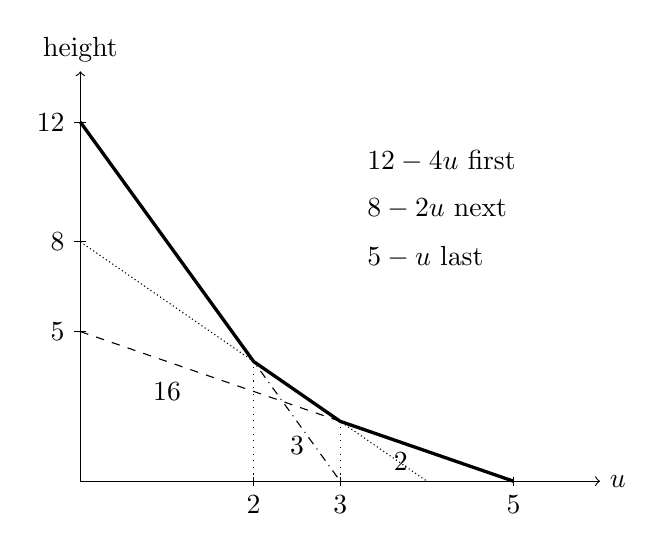
\begin{tikzpicture}[x=1.1cm,y=.38cm]
 \draw[->] (0,0)--(6,0) node[right] {$u$};
 \draw[->] (0,0)--(0,13.7) node[above] {height};
 \draw[dashed] (0,5)--(5,0);
 \draw[densely dotted] (0,8)--(4,0);
 \draw[dash dot] (0,12)--(3,0);
 \draw[very thick] (0,12)--(2,4)--(3,2)--(5,0);
 \draw[dotted] (2,0)--(2,4);
 \draw[dotted] (3,0)--(3,2);
 \foreach \x in {2,3,5}{\draw (\x,.15)--(\x,-.15) node[below] {$\x$};}
 \foreach \y in {5,8,12}{\draw (.07,\y)--(-.07,\y) node[left] {$\y$};}
 \node at (1.0,3) {$16$};
 \node at (2.5,1.2) {$3$};
 \node at (3.7,.65) {$2$};
 \node[anchor=west] at (3.2,10.7) {$12-4u$ first};
 \node[anchor=west] at (3.2,9.1) {$8-2u$ next};
 \node[anchor=west] at (3.2,7.5) {$5-u$ last};
\end{tikzpicture}
\caption{The envelope at the exact saddle $s^*=(5,8,12)$.
The numbers inside the three regions are their areas, not measured data.}
\label{fig:envelope}
\end{figure}

For derivative index $\alpha=k(2,1,2)$, the saddle is
$k(5,8,12)$ and the quadratic cost is $21k^2$. This is the family used in
the numerical diagnostics below.

\subsection{The classical one-dimensional dyadic check}

Arias de Reyna's derivative identity for the normalized up-function
$\operatorname{up}$ on $[-1,1]$ gives
\begin{equation}
 \norm{\operatorname{up}^{(n)}}_\infty=2^{n(n+1)/2}
 \label{eq:upnorm}
\end{equation}
from its translated, signed copies with maximum magnitude one
\cite[Theorem 4]{Arias}. In our centered normalization with $q=1/2$,
$Y/2$ has the up-density, hence
\begin{equation}
 f(y)=\tfrac12\operatorname{up}(y/2),\qquad
 \norm{f^{(n)}}_\infty=2^{(n^2-n)/2-1}.
 \label{eq:knowncheck}
\end{equation}
Its logarithmic leading term is $(\log2)n^2/2$, as required.
Equation \eqref{eq:knowncheck} is a consistency check against a classical
special case, not a claimed new result.

\section{Verification, reproducibility, and the formalization boundary}
\label{sec:verification}

\subsection{Exact finite checks}

The script \texttt{code/verify.py} uses rational arithmetic for the finite
convex geometry. With a fixed seed, it tests 1,200 parameter/order cases in
dimensions one through six. Each case checks seven statements: equality
$\He(Ma)=\Qf(a)$; the identity $a\cdot Ma=2\Qf(a)$; the Fenchel inequality
at an independently chosen scale; degree-two homogeneity; the tail-sum
formula \eqref{eq:costtail}; the determinant \eqref{eq:detM}; and the
isotropic domination $\Qf(a)\le\lambda_{\max}|a|^2/2$.

The envelope integral is computed independently by enumerating pairwise line
crossings and integrating the winning line on each interval. Thus the check
does not merely evaluate the same quadratic formula twice. It also checks
100 signed-parity coefficient cases, with two exact assertions in each case,
and the worked area value $21$. All 8,601 exact assertions passed.
These finite checks are useful error detectors; the general proofs remain
the analytic and algebraic arguments in the article.

\subsection{High-precision product diagnostics}

The numerical run used Python 3.13.5, mpmath 1.3.0, and 160 decimal digits.
Each of five logarithmic boxes and eight ray windows was sampled at 96
reproducibly generated points. These samples are diagnostics, not a proof of
the mean inequalities or a numerical optimization certificate.

The omitted product tail is bounded using \eqref{eq:sinc-tail}:
if the next coefficient vector is $b$ and $r=\max_j|q_j|$, then once
$\sum_j|b_j|\le1$,
\begin{equation}
 0\le-\log\left|\prod_{k\text{ in tail}}\sinc A_k\right|
      \le\frac{(\sum_j|b_j|)^2}{5(1-r^2)}.
 \label{eq:numericaltail}
\end{equation}
The largest evaluated tail bound in the box and ray runs was below
$10^{-90}$. This bounds truncation analytically but does \emph{not} enclose
floating-point rounding error; the computations are not interval-certified.
The signed factorization \eqref{eq:resfourier} was also tested numerically,
with maximum discrepancy in logarithms below $4.6\times10^{-101}$.

\begin{table}[htbp]
\centering\small
\begin{tabular}{rrrrr}
\toprule
$k$ & $|\alpha|$ & $\Qf(\alpha)$ & Sample mean $\log|\Phi|$ & Best log witness\\
\midrule
1 & 5 & 21 & -35.450 & 9.200 \\
2 & 10 & 84 & -110.071 & 64.985 \\
4 & 20 & 336 & -384.602 & 300.770 \\
8 & 40 & 1344 & -1438.377 & 1274.007 \\
16 & 80 & 5376 & -5562.780 & 5233.148 \\
\bottomrule
\end{tabular}

\caption{The family $\lambda=(1,2,4)$, $\alpha=k(2,1,2)$.
The witness is $\sum_j\alpha_j\log t_j+\log|\Phi(t)|-\log W$, with the
omitted-tail loss subtracted. Analytically it lower-bounds the logarithm of
every $L^p$ derivative norm at that frequency; the displayed numerical
values themselves have not been interval-enclosed.}
\label{tab:diagnostics}
\end{table}

The files \texttt{box\_diagnostics.csv} and \texttt{ray\_diagnostics.csv}
preserve more digits and additional normalized errors. The verification
report records versions, precision, counts, and the numerical status.

\subsection{A feasible proof-assistant decomposition}

No Lean or Rocq file is supplied, and none of the new analytic theorems is
claimed to be kernel-checked. A useful formalization order would be the
following. First prove the finite matrix factorization and the tail-sum
quadratic identity. Next formalize the line-envelope integral, the exact
conjugacy inequality, and the attaining scale $Ma$. Those statements have
short finite-dimensional dependencies and are independently valuable.

The analytic stage should separate the one-factor logarithmic integral from
the infinite product. It needs the integrability of $\log|\sin|$ over compact
intervals, the conditional uniform-interval calculation, and Tonelli for
nonnegative negative logarithms. The uniform upper estimate then requires
only a finite bad-index bound and sum--integral comparison. Fourier inversion,
compact support, and H\"older yield the derivative theorem.

Finally, the parity factorization and fixed-order parameter-continuity lemma
should be proved independently before connecting them to the noncommuting
limits. This ordering prevents a proof from silently reusing the
nonresonant estimate at a resonant parameter, where that estimate is false.

\section{Further research questions}
\label{sec:questions}

The main quadratic smoothness problem is settled above under
\eqref{eq:assumptions}. The next questions concern finer information or
regimes deliberately excluded from the theorem.

\begin{question}[The linear-order derivative profile]
For a fixed rational direction $a\ge0$, determine the behavior of
\[
 \log\norm{\partial^{na}f}_p-n^2\Qf(a)
\]
on admissible integer subsequences. Is there a linear term with a limit
coefficient, an order-$n$ oscillation, or a dependence on $p$ at that scale?
The classical dyadic one-dimensional formula shows that an exact linear
term can exist, but it does not determine the coupled case.
\end{question}

\begin{question}[A distributional refinement of the Fourier envelope]
Let a frequency be uniform in a box $B_{ns}$. Study the centered logarithm
$\log|\Phi(t)|+n^2\He(s)$ after division by $n$ or by a smaller fluctuation
scale. This asks for genuine joint sine-product statistics, beyond the
first-moment argument used here. It is also the proper place to assess the
repository's periodic/quasiperiodic remainder proposal rather than treating
it as a consequence of the leading envelope.
\end{question}

\begin{question}[The near-opposite-parameter crossover]
For $(r,-re^{-\varepsilon})$, find a uniform formula when the derivative order
and $\varepsilon^{-1}$ both grow. The two limiting quadratic coefficients are
now known exactly. When $\varepsilon$ is exponentially small in the order,
odd-digit Fourier factors can remain effectively suppressed over a substantial
range. Determine the correct transition variables and the resulting
interpolating quadratic profile; no crossover formula is proved here.
\end{question}

\begin{question}[Confluent jets]
When positive parameters coalesce, divided differences lead to coefficient
vectors involving $k^mq^k$. Determine the sharp mixed-derivative law in a
nonsingular jet coordinate system, including possible order-$n\log n$
corrections caused by polynomial factors. Taking the limit of $M$ alone is
not sufficient, because the coordinate transformation becomes singular.
\end{question}

\begin{question}[Complex parameters and residue-class resonances]
For parameters $re^{\ii\theta_j}$, view the law in its real span and classify
how rational phase differences split digits into residue classes. The pair
$r,-r$ is the period-two example. For irrational phases, cancellation is no
longer confined by distinct real exponential slopes, and a replacement for
\cref{lem:bad} is needed.
\end{question}

\begin{question}[Other digit distributions]
Replace a uniform digit by a compactly supported distribution whose
characteristic function has a controlled averaged algebraic logarithmic
loss. Formulate necessary and sufficient hypotheses under which the cost
is a scalar multiple of $\Qf$. The exact convolution-power theorem gives one
nontrivial family where the multiplier is known, but arbitrary characteristic
zeros may change the conclusion.
\end{question}

\begin{question}[Local regularity and sharp boundary profiles]
Locate the spatial points at which high mixed derivatives achieve their
large norms. Determine whether the global non-Gevrey conclusion holds on
every interior open set, and classify boundary directions where
\eqref{eq:flatness} has a matching lower bound. Global Fourier witnesses do
not answer either spatial question.
\end{question}

\begin{question}[Effective constants and certified inversion]
Replace the deliberately loose bad-index and sine-average constants with
computable sharp or near-sharp ones. Combine them with interval sine
products and validated multidimensional quadrature to make
\cref{prop:truncation} a practical certificate generator for joint density
values and derivatives.
\end{question}

\begin{question}[Formalization and broader envelope dualities]
Formalize \cref{thm:dual} first, then the analytic bridge to derivative norms.
More generally, identify other random-series coefficient systems for which
a finite-line or finite-cone envelope has an explicit positive-orthant
conjugate. The present example shows that such a conjugate can encode a
complete anisotropic regularity law rather than only a tail estimate.
\end{question}

\section{Conclusion}

The joint smoothness of common-digit Fabius laws is governed by an explicit
finite matrix. The proof passes through three quantitative statements:
a uniform upper bound that loses only finitely many cancellation indices;
a matching lower envelope obtained by integrable sine-log averaging;
and an exact convex conjugacy. Together they determine every mixed
$L^p$ derivative norm up to factors exponential in the total order.

The result both answers a precise version of the repository's sharp Fourier
envelope question and adds information not present in a fixed-ray estimate.
The signed resonance demonstrates why the hypotheses matter: smooth
parameter dependence at every fixed order coexists with a discontinuous
quadratic high-order profile. The remaining questions now concern secondary
terms, local geometry, and transition regimes, rather than an unspecified
leading growth constant.

\appendix
\section{Explicit constants and a reusable proof checklist}
\label{app:constants}

The proofs give actual finite constants, although they are not optimized.
A convenient collection is
\begin{align}
 B_0&=\sum_{i<j}\left(1+\frac{2\log(2d)}{|\lambda_i-\lambda_j|}\right),\\
 C_+&=\log2+B_0+\frac{\log2}{\lambda_{\min}},\\
 C_d&=(1+4\pi d)\log2+\log(2d),\\
 T_0&=\frac1{5(1-e^{-2\lambda_{\min}})},\\
 C_-&=1+C_d\left(1+\frac{1+\log(2d)}{\lambda_{\min}}\right)+T_0.
\end{align}
The last choice dominates the constant and the coefficient of $S$ in
\eqref{eq:explicitmean}. Put $c=2+C_+$ and
\begin{equation}
 A_1=4^d\exp\bigl(C_++c^2\Qf(\one)\bigr),\qquad
 B_1=\exp\left(c\max_j(M\one)_j\right).
\end{equation}
Then \eqref{eq:momentbound} holds with these $A_1,B_1$. For the derivative
lower bound, \eqref{eq:derivlower} supplies
\[
 W^{-1}e^{-C_-}e^{-C_-\lambda_{\max}|\alpha|}e^{\Qf(\alpha)}.
\]
Taking maxima of these constants, and incorporating $(2\pi)^{-d}$ and $W$,
gives the two constants in \cref{thm:main}.

A proof using this framework must keep six distinctions intact:
\begin{enumerate}[leftmargin=2em,label=\arabic*.,noitemsep,parsep=0pt]
 \item Signed parameters may be distinct while their moduli coincide;
       the bounded-transition argument needs distinct moduli.
 \item A Fourier lower envelope is not a pointwise lower bound at every
       frequency; exact zeros cannot be discarded by assertion.
 \item The logarithmic-box averaging variables are shared across factors;
       no independence of different factors is available or needed.
 \item The conjugacy is on nonnegative derivative orders; the envelope is
       not one global quadratic polynomial.
 \item The Fourier witness lower-bounds a norm on the entire support and
       does not locate a spatial maximizer.
 \item The error constants are uniform in derivative orders and $p$, but
       not in vanishing modulus gaps.
\end{enumerate}

\section{Package contents and rebuilding}

The archive contains the TeX/PDF article, verification code, generated data,
a JSON test report, provenance, requirements, and a README. The following
commands run the computations and typeset the article:
\begin{verbatim}
python -m pip install -r requirements.txt
python code/verify.py
pdflatex -interaction=nonstopmode -halt-on-error article.tex
\end{verbatim}
Run the last command three times to resolve references. The included data
also allow PDF rebuilding without rerunning Python. No font files are
redistributed; the README lists the required TeX packages.

\begingroup
\small
\setlength{\parskip}{0pt}
\begin{thebibliography}{9}
\bibitem{Repo}
Vladimir Reshetnikov / ProveIt research corpus,
\emph{Common-Digit Fabius Zonoids: Exact volumes, hyperbolic-secant geometry,
Bernoulli Gaussianization, and parameter jets}.
Unrefereed repository report, inspected at commit
\texttt{23dd71d2d3d5e85d2b97a8cc45f55e735d69a4ae}.
Relevant labels: \texttt{thm:joint-char}, \texttt{thm:density-regularity},
\texttt{conj:ray-decay}.
\href{https://github.com/VladimirReshetnikov/ProveIt/blob/23dd71d2d3d5e85d2b97a8cc45f55e735d69a4ae/Analysis/FabiusFunction/docs/semi-formalized-research-frontiers/drafts/representations/common_digit_fabius_zonoids_frontier_report/common_digit_fabius_zonoids.tex}{Pinned source in the ProveIt repository}.

\bibitem{Fabius}
J. Fabius, \emph{A probabilistic example of a nowhere analytic
$C^\infty$-function}, Zeitschrift f\"ur Wahrscheinlichkeitstheorie und
Verwandte Gebiete \textbf{5} (1966), 173--174.
Institutional preprint record (1965):
\href{https://ir.cwi.nl/pub/8160}{CWI publication 8160}.

\bibitem{Arias}
J. Arias de Reyna, \emph{An infinitely differentiable function with compact
support: Definition and properties}, arXiv:1702.05442 (2017), English
translation of the author's 1982 paper. In particular, Theorems 1--4 for the
compactly supported function, its probability interpretation, and its
explicit derivatives.
\href{https://arxiv.org/abs/1702.05442}{arXiv record}.
\end{thebibliography}
\endgroup
\end{document}
